\section{BMS Architectural Shortcomings for Supporting Emergying Application Development}

\begin{figure}[t!] %htbp
\centering
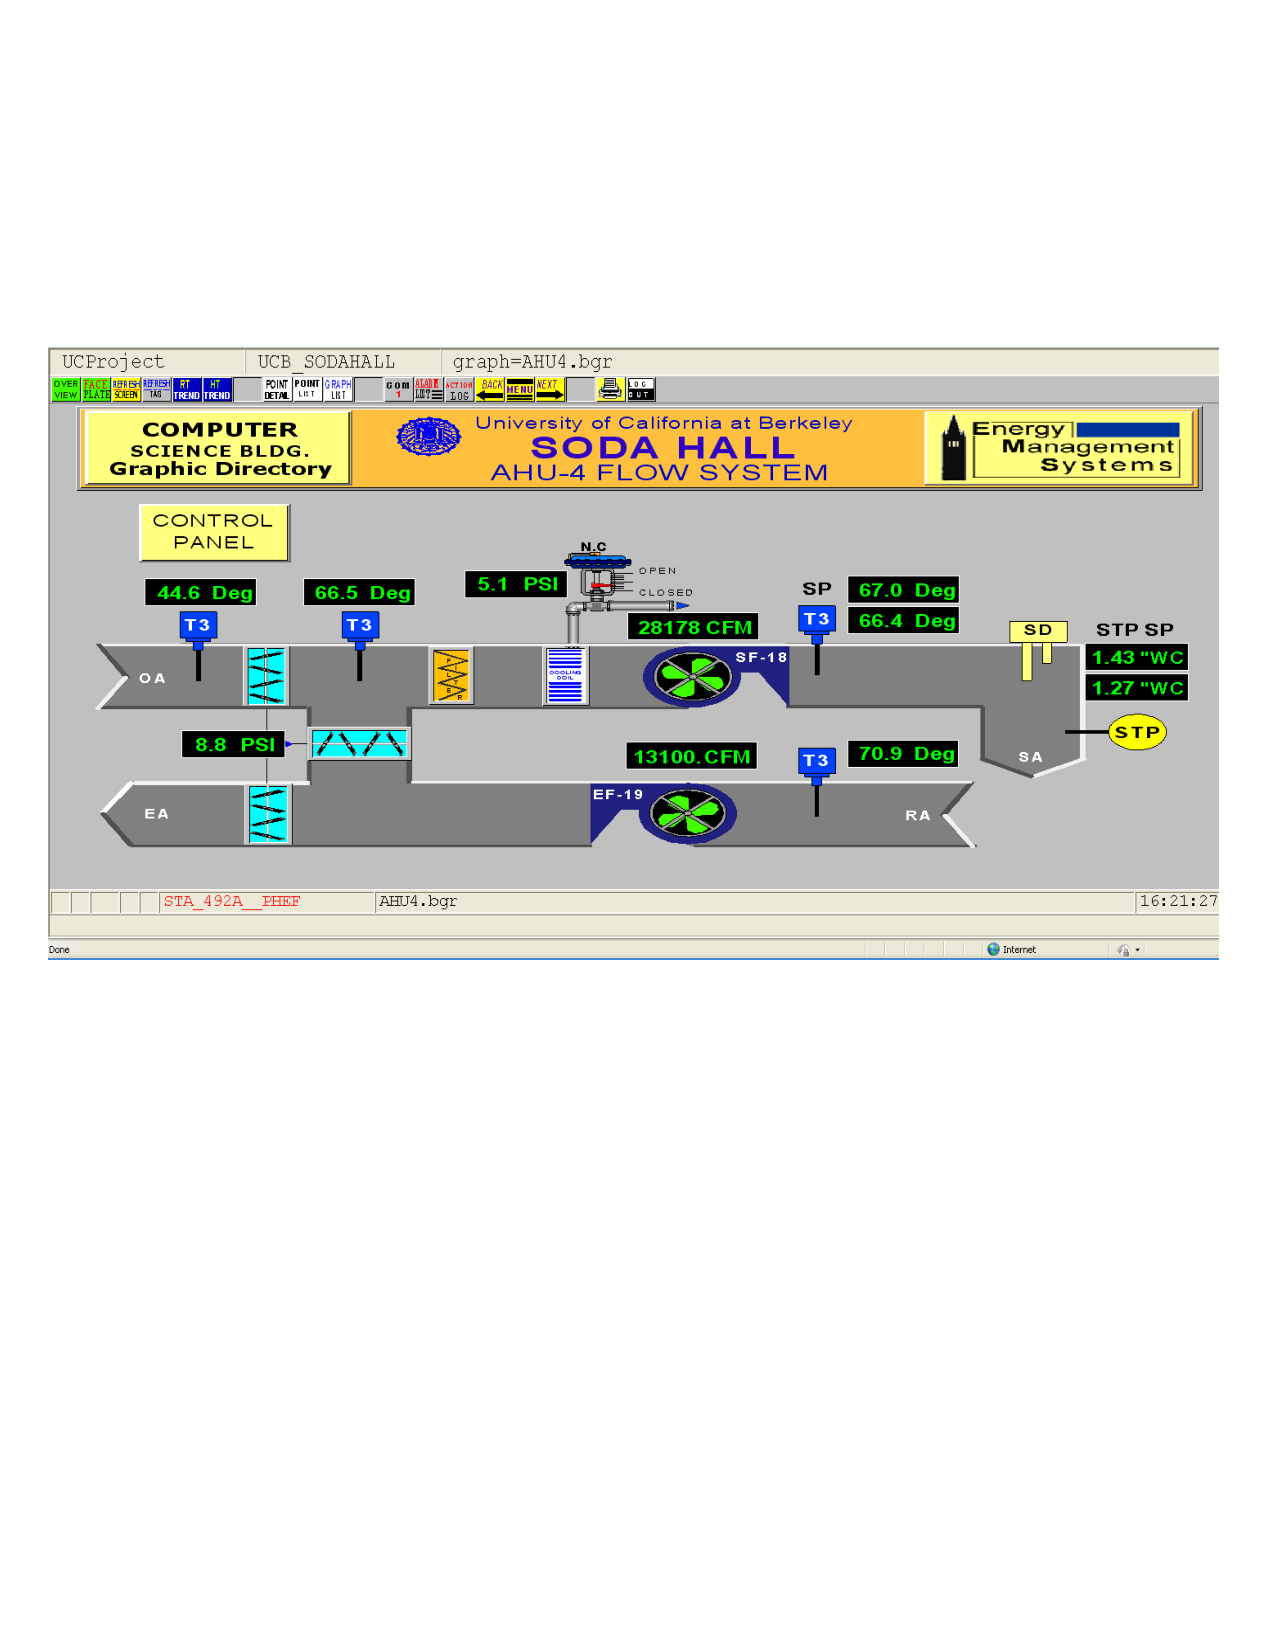
\includegraphics[width=0.75\columnwidth]{figs/soda_bms_screenshot}
\caption{Screen shot for the Soda Hall Building Management System Interface.}
\label{fig:soda_bms_screenshot}
\end{figure}

% In this section we dissect the current architecture in the context of current and future applications
% for buildings.  The first two describe how the current architecture is used to provide the intended service
% that these application provide.  The latter two are emerging applications that we would like to available
% throughout the entire building stock.  We will see, however, that these are very difficult to build at scale
% and we pose the question ``what is missing in the current architecture to enanble the system properties that help
% support these and other emerging applications?''.  Through close inspection it will hopefully become clear that
% the current architecture is fundamentally flawed; built largely to support a small set of vendor-specific
% applications and not much else.

In this section we dissect the BMS architecture and closely examine how well it can support broad application development
in buildings, rather than the single supervisory control function it supports today.  We examine the architecture in the context
of 4 potential services with distinct operational requirements that need to be supported.  The first two services that 
are offered today and enabled by the BMS.  We describe how emerging requirements are driving the evolution of these
services and how BMS's are struggling to meet the new requirements due to limitations in their architectural design.
The next two are emerging services that BMS's cannot support today.  We describe which architectural components must be included
or how current components must be modified in order to support these.  We also make the broader argument that 
building systems should be built to support a much wider range of applications that we cannot currently anticipate.
We will show why this requires a fundamental re-design and propose an architectural composition for such a system.
In the rest of the thesis, we will examine an instance of our architecture and describe the challenges in realizing
the use and effectiveness of our system in real building deployments.

% while the latter are potential applications we imagine will be supported in future
% smart buildings.  Through this exercise, we build our argument for a systematic re-design of such systems and propose
% a set of necessary architectural components necessary to enable and support emerging applications.

\subsection{Monitoring and Supervisory Control}
The primary objective in the design of building information systems is for centralized monitoring and supervisor
control.  Control algorithms are left ``to the expert'' and embedded in the outstation control board.  The intended
user of the system is a building manager -- a user whose expertise is more high-level than control-algorithm or system specific.
The manager is expected to monitor the health of building systems and quickly diagnose problems when they occur.  The tool
is mainly in place to save the building manager time; and it is very effective at doing so.  The extent to which 
the building manager is making control decisions is altering control algorithm paramter setting through
the building management interface itself.  Even these decisions typically go through the vendor, through consultation.

Figure~\ref{fig:soda_bms_screenshot} shows a screenshot of the BMS in Soda Hall at UC Berkeley.  This specific image
captures a schematic for one of the air handling units.  It shows the various sensors embedded in different locations
on the component -- on either side of the supply/exhaust fans, temperature sensors at the supply/return sides of the
air ducts and the inlet vent, measuring the outside air temperature.  Accompanying real-time readings are juxtaposed
by the sensor image.  The user can double-click on the sensor or reading to get more information about that particular 
measurement point.  For example, if you double-click on a temperature sensor, it will give you the exact name of the 
point and accompanying information about related points, such as the set-point, which effectively drives the behavior of 
the underlying system.  If an occupant makes a complaint about not getting any air from the vents, for example, the 
building manager can find the screen for the vents that serve the room the occpant is in and observe the current
pressure readings or look for value-based alerts on any of the readings, typically displayed on the same screen.
If there is a malfunctioning component or something stuck in the vent, the readings should ``look off'' to the building 
manager.

If the problem recurs often, the astute building manager may be able to characterize the fault through a series of alarms.
They can be proactive about finding and fixing the problem(s) before they occur.  Alarms can be set through interaction
with the graphical interface, in much the same way that a lookup on the measurement point occurs -- by double-clicking on 
the point in question and following instructions for setting an alarm.  In some cases, the problem may be driven 
by a faulty setting and adjustments can be made to the control parameters through the associated control points.

The scope of control is limited to specific control loops.  Recall our discussion of control loops in section~\ref{sec:control_loops}.
The building manager can, typically with the help of the vendor, decide on the best control strategy setting.  If the control
strategy cannot be met, due to flaws in the control algorithm itself, the vendor may step in and re-image the controller
at the outstation and expose the necessary parameters through the graphical interface.  These kinds of changes are rare
but do happen occassionally and can be somewhat expensive, since the cost is not typically included with the purchase
of the system.  Because of the cost, the decision is typically made after close inspection and analysis, which a typical BMS
enables.  For example, the sense/control points in question may be placed in ``trend'' mode.  This means that readings
from those streams are stored in the local memory buffer at the outstation for some period of time.  If a report is specifically
set up at the central system, a report period if also associated with the point, allowing the saved points to be drained
from the local buffer at the outstation.  The points are then placed in a file for observation and graphing by the 
building manager.  Time-dependent inspection of the behavior of any of the control-loop related points can be examined.

Although this feature is not necessary in order to change control paramters, it is useful for observing how parameter changes
affect the behavior of the system.  The building manager can, in principal, experiment with different setting and allow
empirical observations to guide her future decisions.


\subsection{Energy Auditing and Building Modeling}
Recently there has been renewed interest in the energy consumption of buildings.  In particular, several studies~\cite{BuildingEnergyData,
MITBuildingScience} show that buildings consome a large fraction of the energy produced in the United States and that as much
as 80\% of it is wasted.  As such, there has been an emergence of several companies and services for assessning the health of
commercial buildings with respect to their energy consumption.  Organizations such as LEED~\cite{Leed} provide certification of 
buildings, specifically rating the energy efficiency of the building.

Building modeling has been part of building science for quite some time, with systems such as EnergyPlus~\cite{EnergyPlus}.
EnergyPlus and simulators like it are part of a larger ecosystem of software for modeling various aspect of the operation
of the building.  They allow the designer to construct detailed models of the building, from construction to usage.  You can
model everything from the material, location, zone-based usage (office building, bathroom, storage room), window size and its
construction, etc.  There are different types of LEED certification, but typical certification requires the submission of the detailed
model and the results of various energy-related metrics, aggregated over seasonal time intervals to attain LEED certification.

Detailed model construction can take several months and in order to ground the underlying model in empirical performance data
typically a modeler will use the data obtained from the building's BMS.  Most vendors provide a way to export the point-related 
trended data.  Complex models can be built using this information.  The file export feature in combination with the ability to 
``trend'' points provide an interface mechanism for these and other kinds of applications that need to make use of the data.

Another option is to obtain the data directly from the system through the network.  Third-party vendors provide systems that 
will join the building network of devices and eavesdrop of the readings and traffic being reported to the central server.
This is the only way to obtain truly real-time readings from the sensors on the network.
Typically BMS vendors do not like this since they may generate too much traffic and overwhelm the network because of congestion.
Although not fundamental, it is a common concern in buildings today.  Many buildings use RS-485 rather than ethernet and there is
a general, albeit unfounded, concern that the network will become overwhelmed if all the points are trended and report at the same
time.

Building modeling and real-time analysis have been separated because of these constraints.  The constraints are largely not
fundamental, but the current architecture is simply not designed to provide real-time readings for \emph{all the points, simultaneously}.
Also, it is clear, even from the fairly simple workloads generated by these analysis applications, that a history of readings
is needed.  BMS's, as currently designed, require the end-user to manage the history of the data point individually.
When BMS's were first designed, there were certainly concerns about bandwidth and storage limits.  However, today those concerns
are a non-issue.  A few hundred bytes produced on the order of a few minutes, even from several thousand sensors is simply not
that much data.


\subsection{Holistic Building Optimization}

\begin{figure}[t!] %htbp
\centering
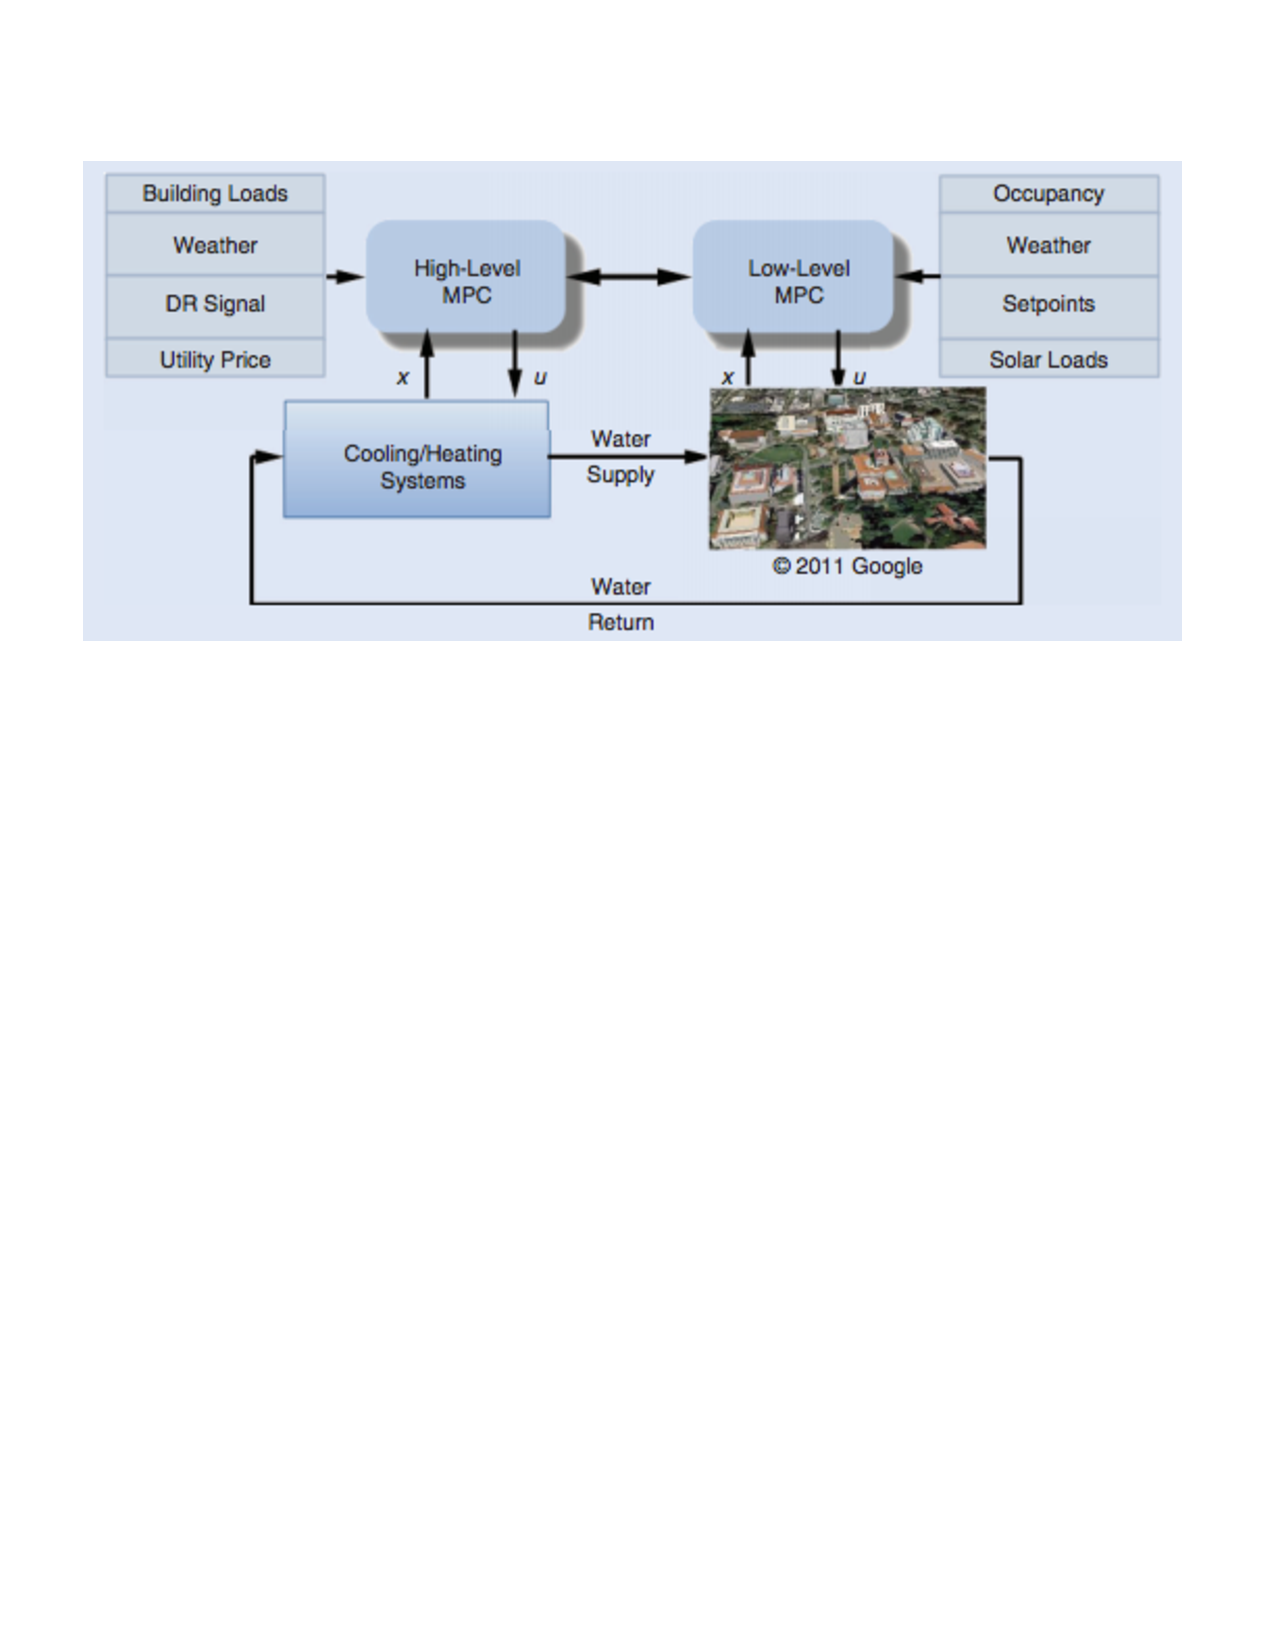
\includegraphics[width=0.75\columnwidth]{figs/mpc1}
\caption{Emerging Application: Hierachical MPC for a stock of buildings.}
\label{fig:mpc1}
\end{figure}

An emerging class of applications, is in holistic control of the building using a new technique called model-predictive control~\cite{MPC}.
Rather than rely on specific changes to control logic at the local-loop level, MPC techniques observe and learn a model
of the behavior of a components, multiple components, or the whole building, based on the historical data.  Once the model is learned, 
constraints can be specified to drive the behavior of the system to an optimal region in the tradeoff space; solving it as 
a constraint optimization problem.  Figure~\ref{fig:mpc1}, reproduced from~\cite{MPC}, shows an example of the how MPC combines 
several points in the building to control the building.  Essentially it decomposes a large optimization problem into indivial control 
decision to be made at the control-loop level.

In order to build this application, the set of necessary points must be mapped into the process.  The user, setting up the problem,
must connect the right data streams and control points to the algorithm by either manually going through the schematics or
locating the schematic representation in the BMS graphical interface.  There is no query interface and it requires that you sit
with the building manager or vendor in order to set up the trending, reporting, and enable the necessary control permisions.
The process is time consuming and \emph{does not scale}.

Although the method is very useful and has yielded excellent results, it is difficult to replicate.  The code and setup must be 
customized for each building or stock of buildings it is set up on.  This lack of generalizability and scalability is missing
in the current state of the art of building information systems.  In most cases the representation of sensor/actuator association is 
implicitly represented in a combination of the schematics, the graphical interface, and the point name.  Moreover, all
three of these change from building to building.  It is fundamentally difficult to generalize.  Buildings are treated as one-off constructions
and their associated digital information has historically followed the same principle.


\subsection{Personal Energy Viewer}
\label{sec:mobile}

\begin{figure}[h!] %htbp
\centering
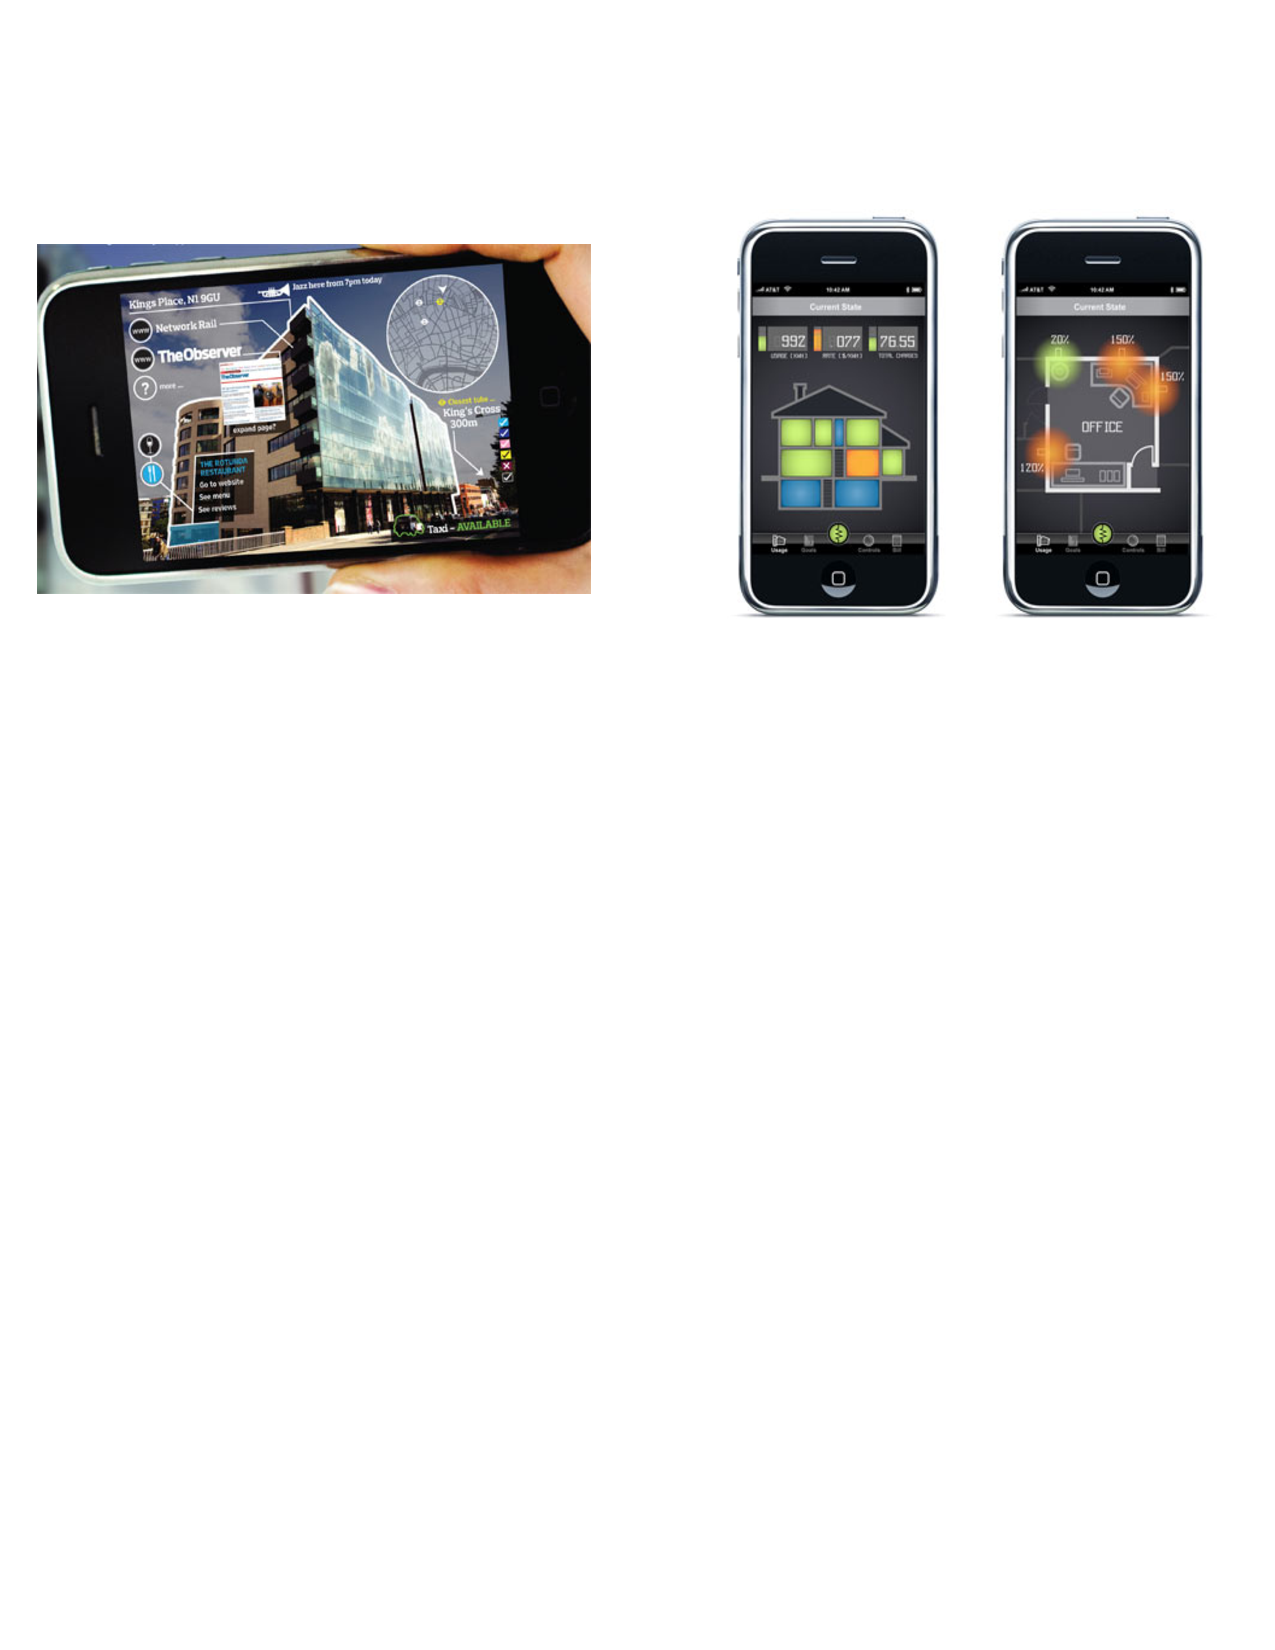
\includegraphics[width=0.75\columnwidth]{figs/mobileEnergy1}
\caption{Emerging Application: Mobile phone interfacing with the physical infrastructure.}
\label{fig:mobileEnergy1}
\end{figure}

Mobile phone penetration continues to rise and is predicted to reach 50 billion by 2020~\cite{mobile2020}.  As such, it is a ubiquitous,
powerful tool to serve as an interface between occupants and the built environment.  Mobile phones are constantly connected, 
are personal devices that can serve as a proxy for the individual, and provide large viewing screen for display of critical information
to its owner.  By combining the data streams available in the building with mobile phone, we could provide a way to
do in-situ diagnosis of opertional problem in the building, monitor personal energy consumption, and share information about
the building with our neighbors in the building.

Currently, in order to enable this application, a detailed digital model of the building is necessary, data streams from the building must
be easy to query, and it should work across buildings.  Also, there needs to be a way to localize the user. 
Localization technology and information must be made available to the mobile application to provide in-situ services.
It's clear that the current information instrastructure cannot provide these.  The interface to the network does not have
a strict naming mechanism, there is not explicit representation of each building that the application could interpret, 
the sensor/actuator deployment is not dense enough and adding new sensor is cumbersome.  Furthermore, the data itself can be quite dirty.

Cheap sensors are unreliable.  They produce erroneous data and randomly stop and start at times.  Missing/errorneous data is common.
Moreoever, within building information systems provided by a single vendor, there is no time synchronization across sensors, so
aggregation, filtering, and re-sampling are common operations that must be performed on the data in order to summarize and display it.
The mobile energy viewer application not only require these but requires that they be performed in real time.


